\documentclass[main.tex]{subfiles}
\begin{document}

\title{
    \textbf{Algorytmy ewolucyjne i metaheurystyki}\\ 
    \begin{large} 
        Sprawozdanie 1
    \end{large}
}

\author{
    Górka Bartosz\\
  \texttt{127228}
  \and
  Zimniak Kajetan\\
  \texttt{127229}
}

\date{}

\maketitle

\section{Opis problemu}
\label{section:opis-problemu}
Celem projektu było przygotowanie dwóch wersji algorytmów rozwiązujących problem grupowania. Liczba grup została ustalona na $10$. Funkcja celu została zdefiniowana jako \textit{minimalizacja średniej odległości wszystkich par obiektów umieszczonych w ramach tej samej grupy}.

Jako kluczowe było wykorzystanie macierzy odległości (dystansu pomiędzy punktami) zamiast użycia przestrzeni kartezjańskiej jako punktu wyjścia. Takie założenie pozwala wykorzystać algorytmy również w przypadku zmiany funkcji odległości (macierz odległości jest wystarczająca do dokonania przydziału).

W rozdziale \ref{section:pseudokody} zaprezentowano pseudokody przygotowanych algorytmów, natomiast w rozdziale\leavevmode\nobreak\ \ref{section:wyniki} wyniki działania algorytmów dla 100 iteracji. Ostatni rozdział dotyczy wizualizacji najlepszych uzyskanych rozwiązań.

\section{Pseudokody przygotowanych algorytmów}
\label{section:pseudokody}
\subsection{Algorytm zachłanny}
\begin{verbatim}
Dla każdego punktu p z listy punktów {
    Dla każdej grupy g z listy grup {
        Sprawdź wartość odległości między punktem p, a elementem startowym grupy g
        
        Jeżeli odległość mniejsza od aktualnie najmniejszej {
            Zapisz odległość jako najmniejszą
            Jako wybraną grupę zapisz g
        }
    }

    Do wybranej grupy z najmniejszym dystansem dodaj punkt p
}
\end{verbatim}

\subsection{Algorytm z wykorzystaniem żalu}
Algorytm z wykorzystaniem żalu dokonuje przydziału obiektu zgodnie z pseudokodem zaprezentowanym poniżej. W każdej iteracji przydziela jeden punkt do jednej grupy. Dla każdego punktu sprawdza jak bardzo jego dołożenie do danej grupy pogorszy wartość funkcji celu. Następnie wybiera punkt, którego dołożenie do którejś z grup będzie najmniej korzystne i dołącza go do grupy, która znajduje się najbliżej niego (najkorzystniejszy wybór wśród wszystkich grup). Inicjalizacja punktów startowych odbywa się poprzez losowy wybór elementu startowego w każdej z grup.

\begin{verbatim}
Dopóki nie przydzielono wszystkich punktów {
    Dla każdego punktu p z listy wszystkich punktów {
        Dla każdej grupy g z listy grup {
            Oblicz średni dystans pomiędzy wszystkimi punktami w grupie g
            Zapisz jak bardzo dodanie punktu zmienia wartość funkcji celu
        }
    }
    
    Wybierz grupę i punkt które mają największą wartość żalu
        (minimalizacja kosztów dodania punktu w kolejnych krokach)
    Dodaj wybrany punkt do wybranej grupy
}
\end{verbatim}

\section{Wyniki eksperymentów obliczeniowych}
\label{section:wyniki}
W tabeli \ref{table:wyniki} zaprezentowano wyniki eksperymentów obliczeniowych. Dokonano $100$ powtórzeń obliczeń, za każdym razem z losowym wyborem elementu startowego w każdej z $10$ grup. Za losowy element startowy uznaje się przydział $10$ różnych punktów do $10$ różnych grup (każda z powstałych grup miała jeden punkt). Przydzielony punkt określany jest punktem startowym grupy.

Obydwa algorytmy wykorzystywały ten sam przydział początkowy grup w ramach pojedynczej iteracji, aby możliwe było ich porównanie.
\begin{table}[H]
\centering
\caption{Wyniki eksperymentów obliczeniowych dla 100 iteracji}
\label{table:wyniki}
\resizebox{\textwidth}{!}{%
\begin{tabular}{|c|r|r|}
\hline
\textbf{Cecha}                                                                     & \multicolumn{1}{c|}{\textbf{Algorytm zachłanny}} & \multicolumn{1}{c|}{\textbf{Algorytm oparty o żal}} \\ \hline
\textbf{\begin{tabular}[c]{@{}c@{}}Wartość minimalna\\ funkcji celu\end{tabular}}  
&   33.92                                               
&   37.62                                                 \\ \hline
\textbf{\begin{tabular}[c]{@{}c@{}}Wartość maksymalna\\ funkcji celu\end{tabular}} 
&   44.44                                              
&   73.82                                                 \\ \hline
\textbf{\begin{tabular}[c]{@{}c@{}}Wartość średnia\\ funkcji celu\end{tabular}}    
&   38.47                                               
&   48.36                                                  \\ \hline
\textbf{\begin{tabular}[c]{@{}c@{}}Wartość minimalna\\ czasu obliczeń {[}sec{]}\end{tabular}} 
&   0,000804                                               
&   0,18                                                  \\ \hline
\textbf{\begin{tabular}[c]{@{}c@{}}Wartość maksymalna\\ czasu obliczeń {[}sec{]}\end{tabular}} 
&   0,029                                               
&   1,52                                                  \\ \hline
\textbf{\begin{tabular}[c]{@{}c@{}}Wartość średnia\\ czasu obliczeń {[}sec{]}\end{tabular}} 
&   0,0017                                               
&   0,258                                                  \\ \hline
\end{tabular}%
}
\end{table}



\section{Wizualizacja najlepszych rozwiązań}
\subsection{Algorytm zachłanny}
\begin{figure}[H]
    \centering
    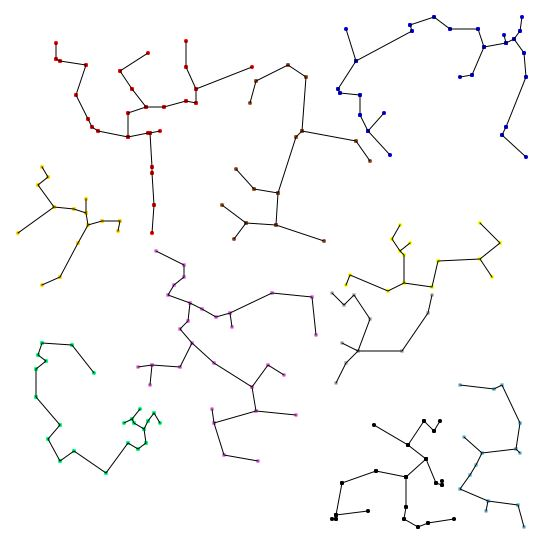
\includegraphics[width=\textwidth]{sprawozdanie_1/zachlanny.png}
    \caption{Algorytm zachłanny - wizualizacja najlepszego przydziału}
\end{figure}

\subsection{Algorytm oparty o żal}
\begin{figure}[H]
    \centering
    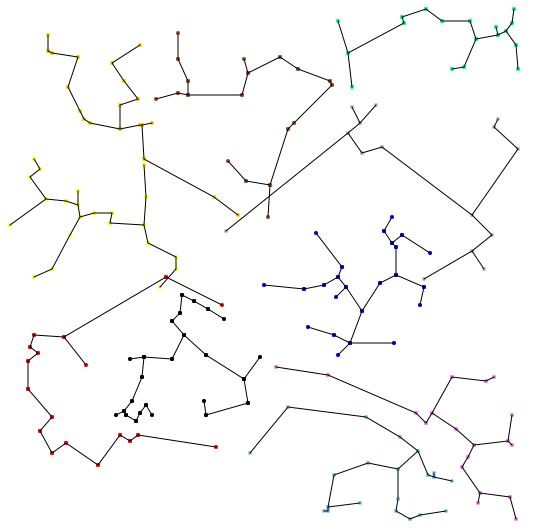
\includegraphics[width=\textwidth]{sprawozdanie_1/regret.png}
    \caption{Algorytm oparty o żal - wizualizacja najlepszego przydziału}
\end{figure}

\end{document}
\end{document}